%----------------------------------------------------------------------------------------
%	PACKAGES AND OTHER DOCUMENT CONFIGURATIONS
%----------------------------------------------------------------------------------------

\documentclass{beamer}
%\usepackage{math}
\usepackage{listings}
%\input{structure.tex} % Include the file specifying the document structure and custom commands

\usetheme{Frankfurt}

%----------------------------------------------------------------------------------------
%	ASSIGNMENT INFORMATION
%----------------------------------------------------------------------------------------

\title{The impact of agent definitions and interactions on multiagent learning for coordination} % Title of the assignment

\author{Authors: Jen Jen Chung, Damjan Miklić, Lorenzo Sabattini, Kagan Tumer, Roland Siegwart
\\ Presentors: Kallinteris Andreas, Orfanoudakis Stavros}

\date{13-2-2019} % University, school and/or department name(s) and a date

%----------------------------------------------------------------------------------------

\begin{document}
	\begin{frame}
		\maketitle % Print the title
	\end{frame}

	\section{Intro}
	\begin{frame}
		\frametitle{Agent Factorization}
		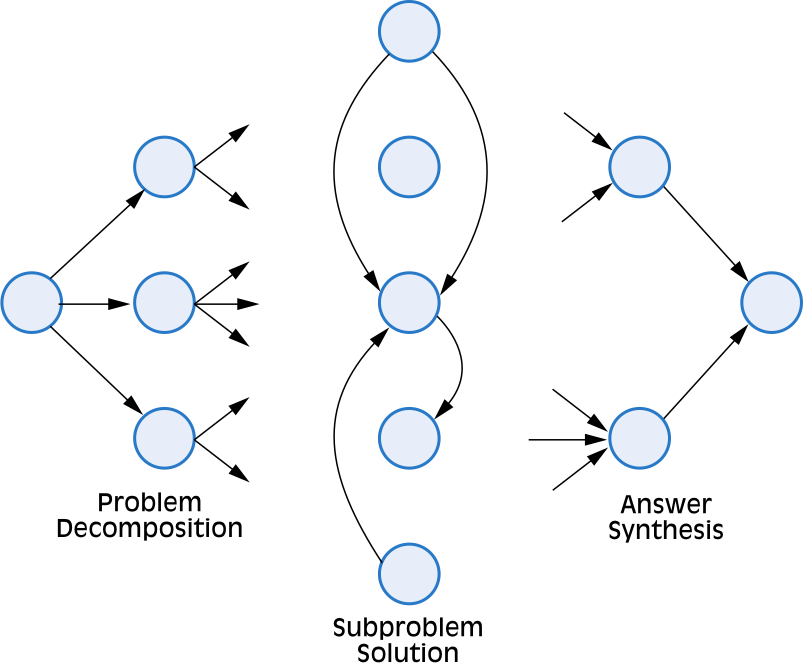
\includegraphics[height=0.9\textheight,width=\textwidth]{agent-factor.png}
	\end{frame}
	\begin{frame}
		\frametitle{Agent Factorization}
		Domains with straight foward agent defintions:
		\begin{itemize}
			\item Robo-soccer
		\end{itemize}
		Domains with easily flexible agent defintions:
		\begin{itemize}
			\item Autonomus Traffic Management
			\item Network Routing
			\item Powerplant Control
		\end{itemize}
		$\Rightarrow$ we can define the optimal agent to learn most efficiently
	\end{frame}
	\begin{frame}
		\frametitle{Agent definition trade-offs}
		%\begin{itemize}
			%\item More Agents $\Rightarrow$ smaller agents (small state/action space) hold a
			%localized view $\Rightarrow$ easy to learn individual policy
			%\item Less Agents $\Rightarrow$ bigger agents (big state/action space) hold a
			%more complete view of the problem
		%\end{itemize}
		\begin{tabular}{|c|c|c|}
		\hline			
		\textbf{Agent Definition Size} & Low Level & High Level \\
		\hline			
		\#Agents & Many & Few \\
		\hline			
		Communication Learn complexity & High & Low \\
		\hline  
		Individual Learn complexity & Low & High \\
		\hline  
		\end{tabular}

	\end{frame}
	\section{Domain}
	\begin{frame}
		\frametitle{Traffic Management Domain}
		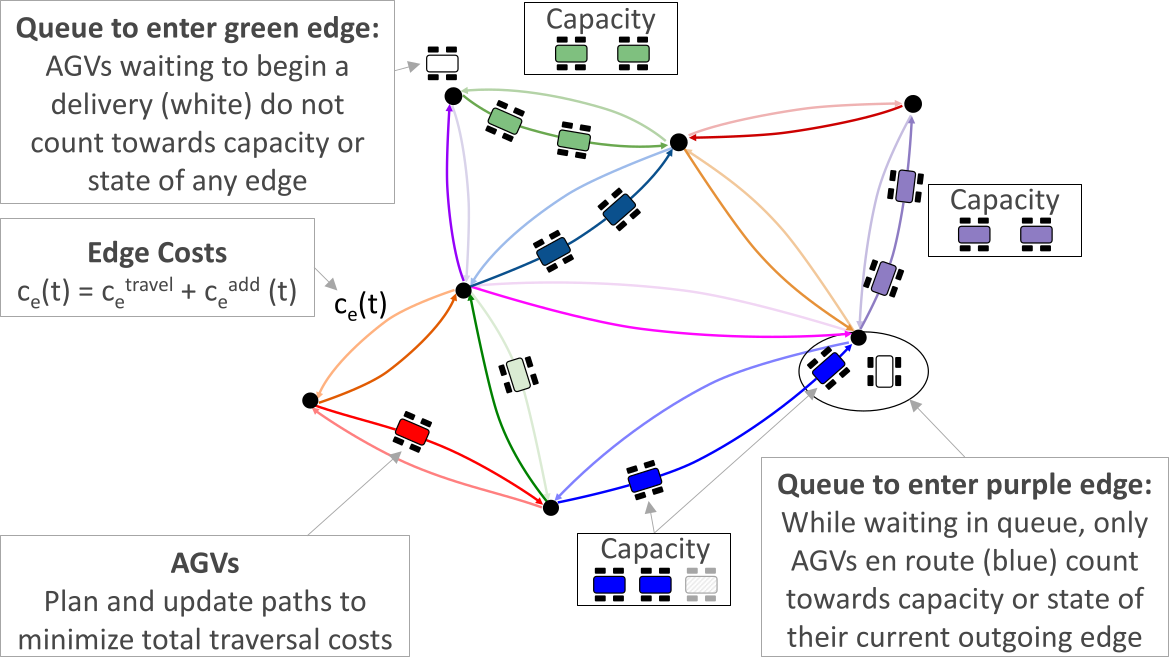
\includegraphics[width=\textwidth]{enviroment.png}
	\end{frame}
	\begin{frame}
		\frametitle{AGV Traffic Management example}
		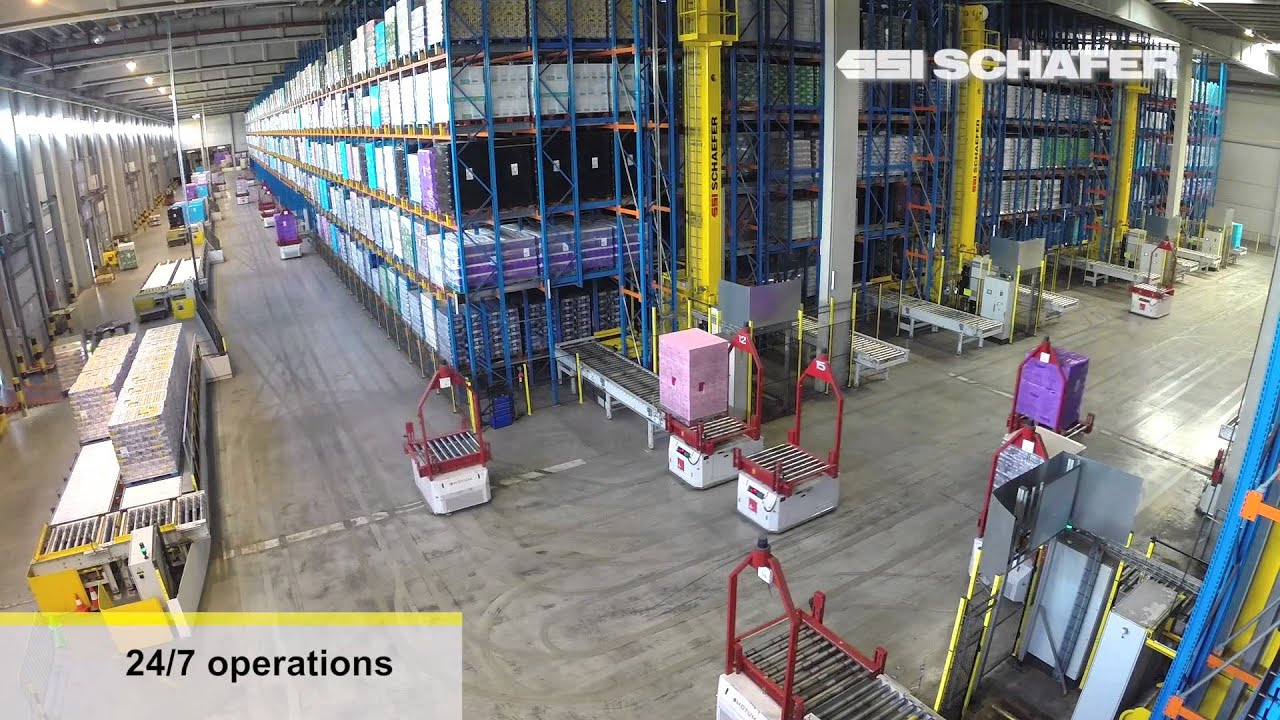
\includegraphics[width=\textwidth]{warehouse.jpg}
	\end{frame}
	\begin{frame}
		\frametitle{Variables (I)}
		Cost for an AGV for traversing an edge
		\begin{itemize}
			\item $cost_e(t) = cost_e^{travel} + cost_e^{add}(t)$
		\end{itemize}
		The Capacity of an edge (based on the physical space)
		\begin{itemize}
			\item $cap_e$
		\end{itemize}
	\end{frame}
	\begin{frame}
		\frametitle{Learning $c_e^{add}(t)$}
		%Problem Complexity too high for real world workload
		%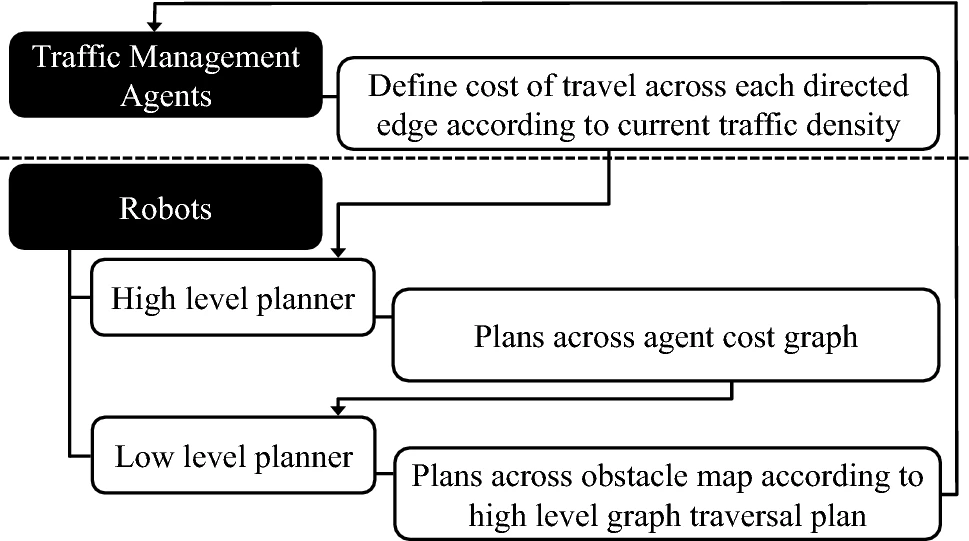
\includegraphics[width=\textwidth]{learn-model.png}
	    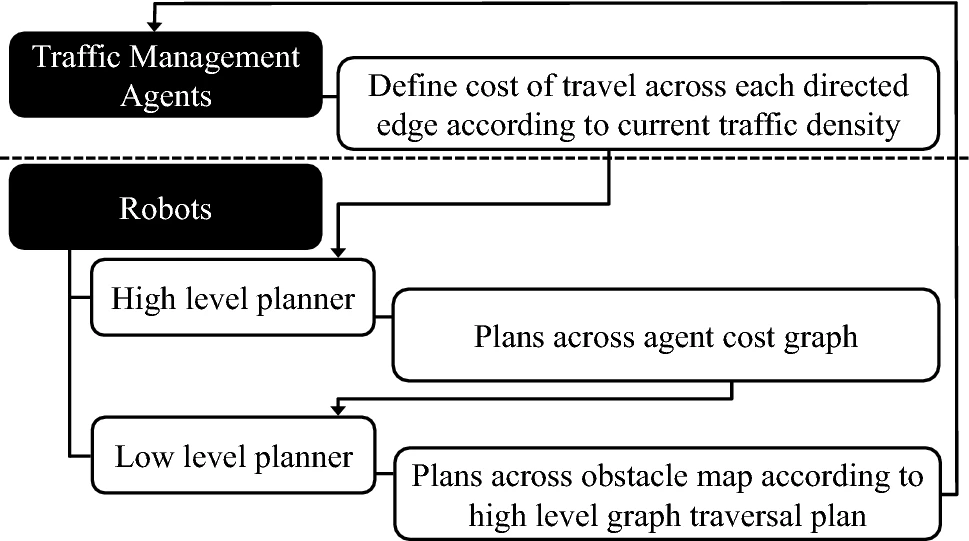
\includegraphics[height=0.9\textheight,width=0.9\textwidth]{learn-model.png}
	\end{frame}
	\begin{frame}
		\frametitle{Variables (II)}
		\begin{itemize}
			\item State of the agents\\ $S_i(t) = [S_e(t)]$, $\forall e \in \mathcal{E}_i$
    \\.

			\item Action of agents\\ $a_i(t) = \pi(S_e(t)) = [cost_e^{add}(t)]$, $\forall e \in \mathcal{E}_i$
\\.

			\item Object of the agents\\ $max_\Pi G(\Pi)$ = total deliveries
			
		\end{itemize}
	\end{frame}

	\section{Agent Definition}
	\begin{frame}
		\frametitle{Agent types}
		\begin{itemize}
			\item Link Agent
			\item Intersection Agent
			\item Central \\.


			\item Link Time Agent
			\item Intersection Time Agent
			\item Central Time
		\end{itemize}
	\end{frame}
	\begin{frame}
		\frametitle{Link Agent}
		\begin{columns}
		\column{.5\textwidth}
			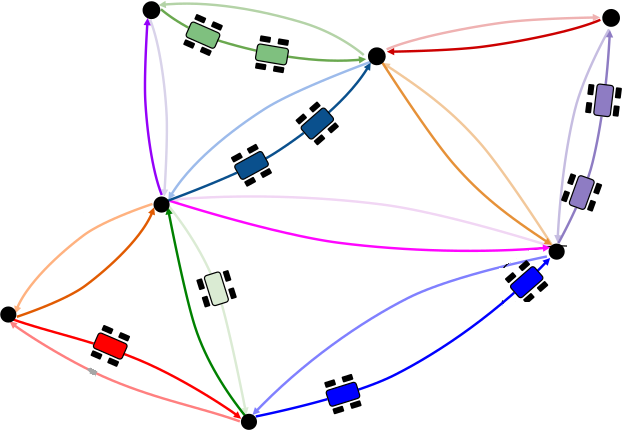
\includegraphics[width=\textwidth]{link.png}
		\column{.5\textwidth}
			Every Link Agent is assigned to in a single directed edge
			\begin{itemize}
				\item $N = |\mathcal{E}|$
				\item $s_i^{link}(t) = n_{e_i}(t)$
				\item $a_i^{link}(t) = c_{e_i}^{add}(t)$
			\end{itemize}
		\end{columns}
	\end{frame}
	\begin{frame}
		\frametitle{Intersection Agent}
		\begin{columns}
		\column{.5\textwidth}
			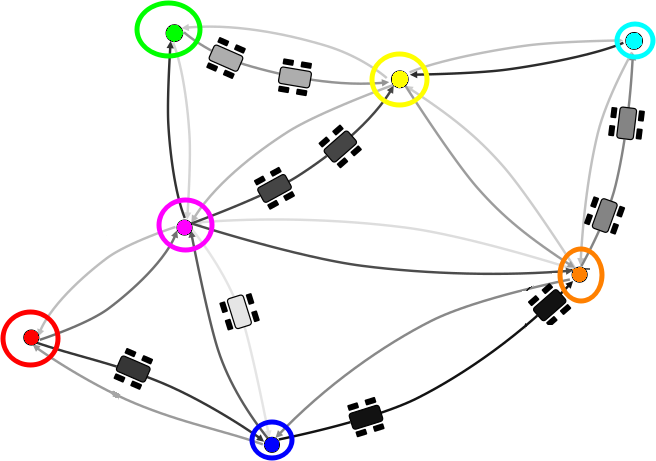
\includegraphics[width=\textwidth]{intersection.png}
		\column{.5\textwidth}
			Every Intersection Agent is assigned to the set of incoming edges of a vertex
			\begin{itemize}
				\item $N = |V| < |\mathcal{E}|$
				\item $s_i^{int}(t) = [n_{e_i}(t)]$, $\forall e \in \mathcal{E}_i$
				\item $a_i^{int}(t) = [c_{e_i}^{add}(t)]$, $\forall e \in \mathcal{E}_i$
			\end{itemize}
		\end{columns}
	\end{frame}
	\begin{frame}
		\frametitle{Agents with incorporated travel time}
		Previous agents + additional state ($d_{e_i}(t)$)
		indicating the remaining time until the latest AGV reaches the vertex \\ .
		\begin{itemize}
			\item $s_i^{link,time}(t) = [n_{e_i}(t), d_{e_i}(t)]$
			\item $a_i^{link,time}(t) = c_{e_i}^{add}(t)$
		\end{itemize}
.
		\begin{itemize}
			\item $s_i^{int,time}(t) = [n_{e_i}(t)], d_{e_i}(t)]$, $\forall e \in \mathcal{E}_i$
			\item $a_i^{int,time}(t) = [c_{e_i}^{add}(t)]$, $\forall e \in \mathcal{E}_i$
		\end{itemize}
	\end{frame}
	\section{Experiment}
	\begin{frame}
	\frametitle{Test Warehouse}
	\begin{center}
    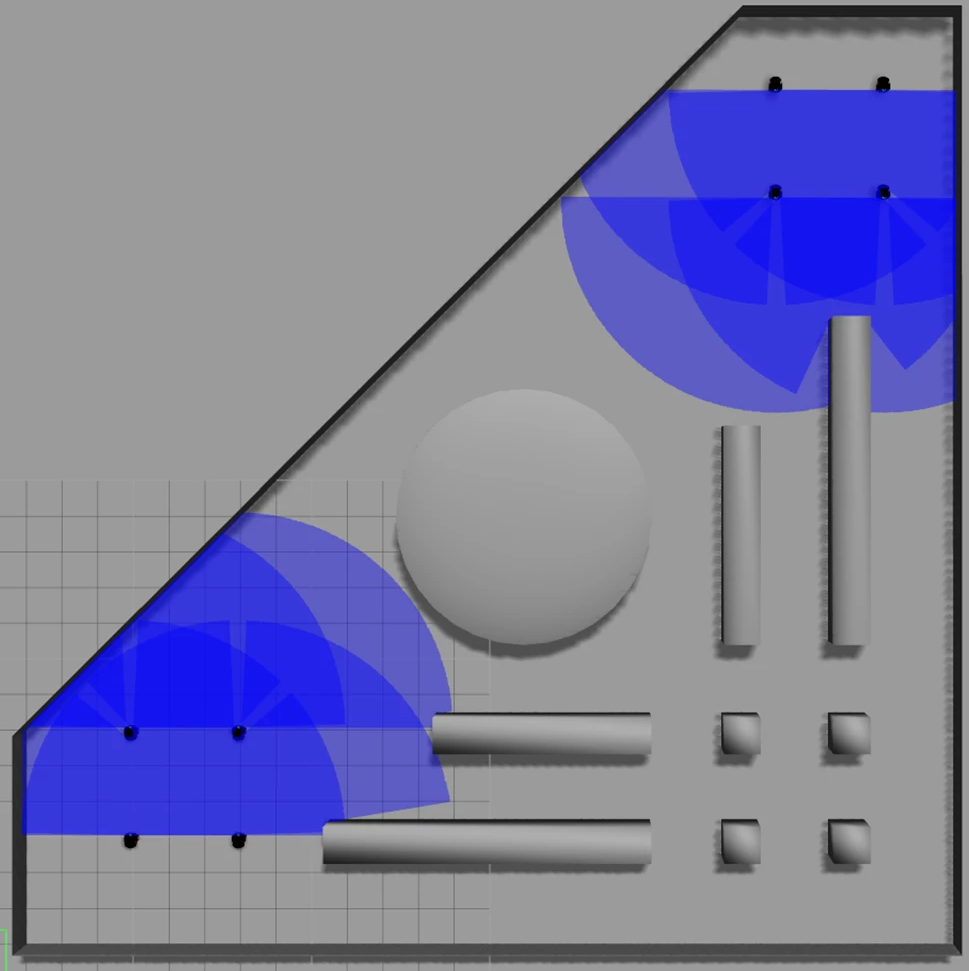
\includegraphics[height=0.9\textheight,width=0.9\textwidth]{exp-r.png}
    \end{center}
	\end{frame}
	
	\begin{frame}
	\frametitle{Simulated Graph of Warehouse}
	\begin{center}
    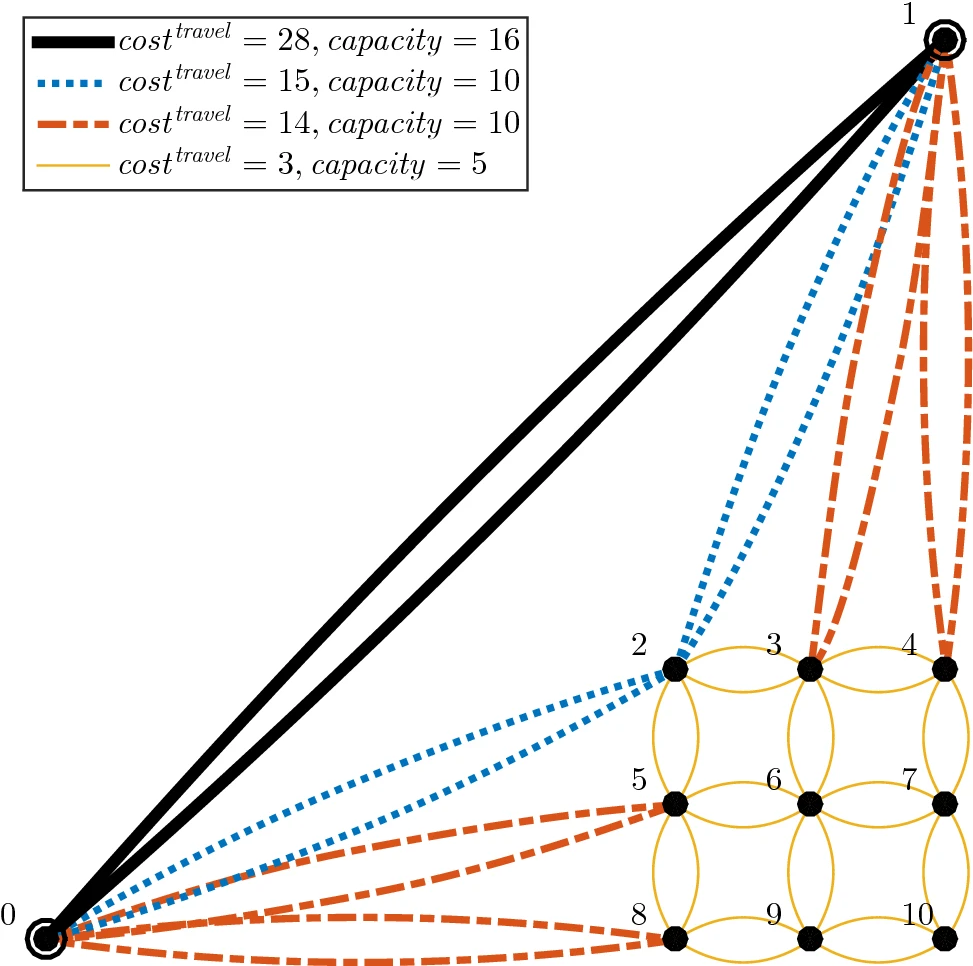
\includegraphics[height=0.9\textheight,width=0.9\textwidth]{exp.png}
	\end{center}
	\end{frame}
	
	\begin{frame}
	\frametitle{Comparison of Agent Definitions}
	\begin{center}
    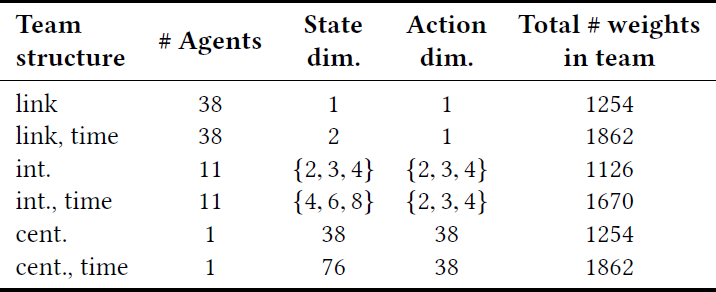
\includegraphics[width=1\textwidth]{comp.png}
	\end{center}
	\end{frame}
	
		\begin{frame}
	\frametitle{Average Team}
	\begin{center}
    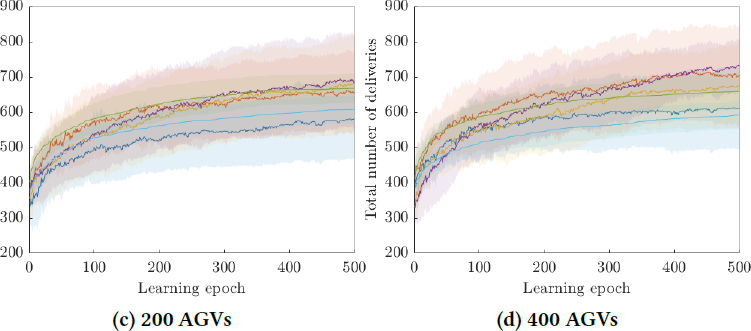
\includegraphics[height=0.425\textheight ]{graph1.png}
    
    
     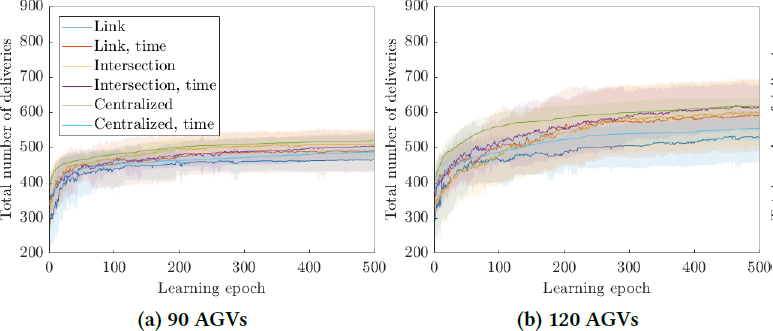
\includegraphics[height=0.425\textheight]{graph2.png}
     \end{center}
	\end{frame}
	
	\begin{frame}
	\frametitle{Performance Distribution}
	\begin{center}
    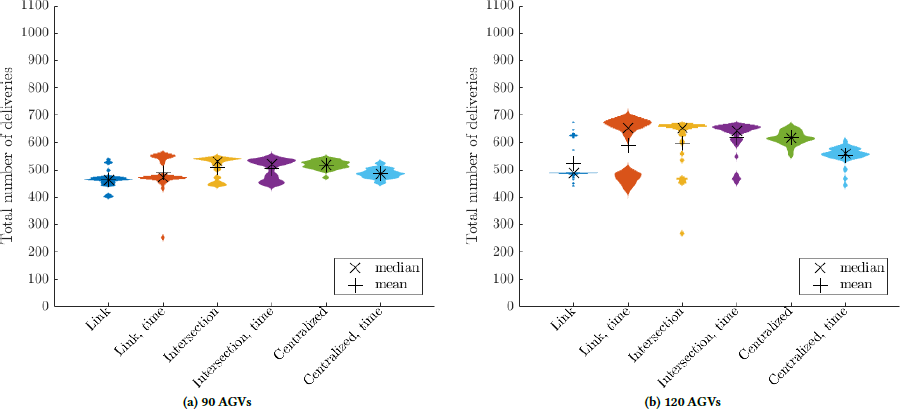
\includegraphics[height=0.425\textheight ]{violin1.png}
    
    
     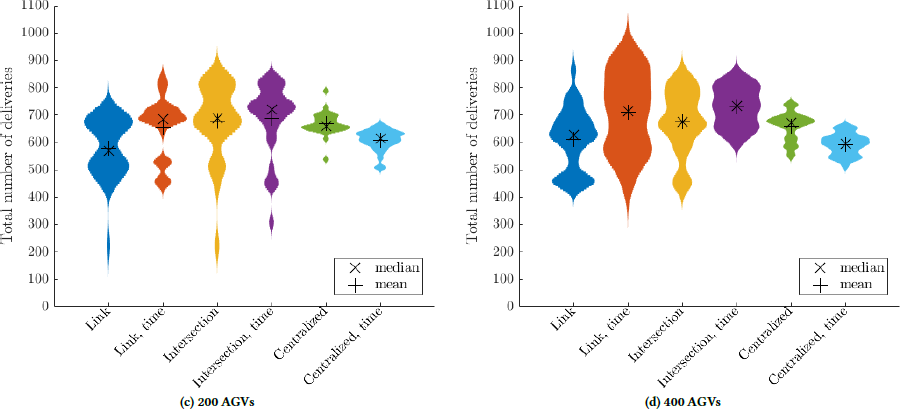
\includegraphics[height=0.425\textheight]{violin2.png}
     \end{center}
	\end{frame}
	
	\begin{frame}
	\frametitle{End}
    Thank you!
	\end{frame}


\end{document}
